\documentclass[12pt, border=3mm]{standalone}
\usepackage{tikz}
\usepackage{tkz-euclide}

\begin{document}
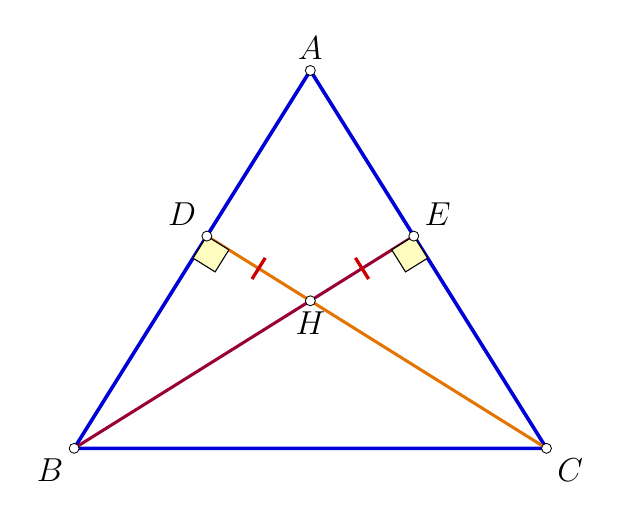
\begin{tikzpicture}[scale=1.5]
    % Định nghĩa các điểm tam giác ABC
    \tkzDefPoint(0, 3.2){A}
    \tkzDefPoint(-2, 0){B}
    \tkzDefPoint(2, 0){C}
    
    % Hình chiếu vuông góc
    \tkzDefPointBy[projection=onto A--B](C) \tkzGetPoint{D}
    \tkzDefPointBy[projection=onto A--C](B) \tkzGetPoint{E}
    
    % Giao điểm H của CD và BE
    \tkzInterLL(B,E)(C,D) \tkzGetPoint{H}
    
    % Styling chuẩn theo phong cách hinh_bai_tap
    \tikzset{
        c_main/.style={thick, color=blue!85!black, line width=1.3pt},
        c_height1/.style={thick, color=orange!90!black, line width=1.1pt},
        c_height2/.style={thick, color=purple!80!black, line width=1.1pt}
    }
    
    % Vẽ tam giác và các đường
    \draw[c_main] (A) -- (B) -- (C) -- cycle;
    \draw[c_height1] (C) -- (D);
    \draw[c_height2] (B) -- (E);
    
    % Đánh dấu góc vuông có fill vàng nhạt (chuẩn hinh_bai_tap)
    \tkzMarkRightAngles[size=0.22, fill=yellow!25](B,D,C C,E,B)
    
    % Đánh dấu 2 đoạn bằng nhau HD = HE
    \tkzMarkSegments[mark=|, size=4.5pt, color=red!80!black, line width=1.2pt](H,D H,E)
    
    % Vẽ các điểm chấm tròn theo phong cách mẫu
    \foreach \p in {A,B,C,D,E,H} {
        \filldraw[fill=white, draw=black, line width=0.3pt] (\p) circle (1.2pt);
    }
    
    % Nhãn đỉnh font toán Computer Modern
    \tkzLabelPoint[above, font=\large](A){$A$}
    \tkzLabelPoint[below left, font=\large](B){$B$}
    \tkzLabelPoint[below right, font=\large](C){$C$}
    \tkzLabelPoint[above left, font=\large](D){$D$}
    \tkzLabelPoint[above right, font=\large](E){$E$}
    \tkzLabelPoint[below, font=\large](H){$H$}
\end{tikzpicture}
\end{document}
